% 
% (c) Copyright 2016 Tabea Mendez
% 
% This source is free: you can redistribute it and/or modify
% it under the terms of the GNU General Public License as published by
% the Free Software Foundation, either version 3 of the License, or
% (at your option) any later version.
% 
% This source is distributed in the hope that it will be useful,
% but WITHOUT ANY WARRANTY; without even the implied warranty of
% MERCHANTABILITY or FITNESS FOR A PARTICULAR PURPOSE.  See the
% GNU General Public License for more details.
% 
% You should have received a copy of the GNU General Public License
% along with this source.  If not, see <http://www.gnu.org/licenses/>.
%
%%%%%%%%%%%%%%%%%%%%%%%%%%%%%%%%%%%%%%%%%%%%%%%%%%%%%%%%%%%%%%%%%%%%%%%%%%%%%%


\newcommand{\db}{\text{dB} }
\newcommand{\dbm}{\text{dBm} }
\newcommand{\dbW}{\text{dBW} }
\newcommand{\dbi}{\text{dBi} }
\newcommand{\lin}{\text{lin} }
\newcommand{\snr}{\text{SNR} }
\newcommand{\khz}{\text{kHz} }
\newcommand{\mhz}{\text{MHz} }
\newcommand{\ghz}{\text{GHz} }
\newcommand{\km}{\text{km} }
\newcommand{\los}{line-of-sight }
\newcommand{\lcr}{\textit{level crossing rate} }
\newcommand{\afd}{\textit{average fade duration} }
\newcommand{\physcalc}{\texttt{physcalc} }
\newcommand{\rawreader}{\texttt{rawreader} }
\DeclareRobustCommand{\myd}{d}
\newcommand{\rot}{\operatorname{rot}}
\newcommand{\grad}{\operatorname{grad}}
\renewcommand{\div}{\operatorname{div}}
\newcommand{\erfc}{\operatorname{erfc}}
\newcommand{\nab}{\vec{\nabla}}
\renewcommand{\d}{\partial}
\DeclareRobustCommand{\e}{\mathrm{e}}
\newcommand{\trace}{\operatorname{tr}}
\newcommand{\Hz}{\text{Hz}}
\newcommand{\sgn}{\text{sgn}}
\DeclareRobustCommand{\E}[1]{
	\operatorname{E}\left[#1\right]
}
\DeclareRobustCommand{\nE}[1]{
	\operatorname{E}#1
}

\DeclareRobustCommand{\var}[1]{
	\operatorname{var}\left[#1\right]
}

\DeclareRobustCommand{\myint}[4]{
	\int\limits
	\ifthenelse{\equal{#1}{}}{}{_{#1}}
	\ifthenelse{\equal{#2}{}}{}{^{#2}}
	#3 \,\myd#4
}

\DeclareRobustCommand{\mysum}[3]{
	\sum\limits
	\ifthenelse{\equal{#1}{}}{}{_{#1}}
	\ifthenelse{\equal{#2}{}}{}{^{#2}}
#3
}

\DeclareRobustCommand{\myprod}[3]{
	\prod\limits
	\ifthenelse{\equal{#1}{}}{}{_{#1}}
	\ifthenelse{\equal{#2}{}}{}{^{#2}}
#3
}

\DeclareRobustCommand{\mylim}[2]{
	\lim\limits
	\ifthenelse{\equal{#1}{}}{}{_{#1}}
#2
}

\DeclareRobustCommand{\myprob}[2]{
	\vspace*{0.1cm}
	\rule[-3pt]{\textwidth }{0.5pt}\vspace*{0.1cm}{\footnotesize\sffamily
	\begin{prob}{Probelm: }
		\item [\bfseries\color{CadetRed} Problem:] {\color{CadetRed} #1}\\[0.1cm]#2
	\end{prob}\vspace*{-0.2cm}}\rule[-3pt]{\textwidth }{0.5pt}\vspace*{0.1cm}
}

\DeclareRobustCommand{\myexam}[2]{
	\vspace*{0.1cm}
	\rule[-3pt]{\textwidth }{0.5pt}\vspace*{0.05cm}{\footnotesize\sffamily
	\begin{prob}{Beispiel: }
		\item [\bfseries\color{CadetRed} Beispiel:] {\color{CadetRed} #1}\\[0.1cm]#2
	\end{prob}\vspace*{-0.5cm}}\rule[-3pt]{\textwidth }{0.5pt}\vspace*{0.2cm}
}

\newenvironment{prob}[1]
{\begin{list}{}
{\renewcommand\makelabel[1]{\textsf{##1}\hfil}
	\settowidth\labelwidth{\makelabel{#1}}
	\setlength\leftmargin{\labelwidth+\labelsep}}}
{\end{list}}

\DeclareRobustCommand{\mybox}[1]{
	\vspace*{0.1cm}
	\begin{center}
		\fcolorbox{white}{black!10}{
	\begin{minipage}{0.90\textwidth}
#1
	\end{minipage}
	\vspace*{0.1cm}
}
	\end{center}
}

\DeclareRobustCommand{\myequation}[2]{
\begin{equation}
#1
\end{equation}
{\begin{center}{\scriptsize{#2}}\end{center}}
}

\usetikzlibrary{calc}
\usetikzlibrary{shapes,snakes}
\usetikzlibrary{arrows,shapes,backgrounds}
\usetikzlibrary{shapes.geometric,shapes.arrows,decorations.pathmorphing}
\usetikzlibrary{matrix,chains,scopes,positioning,arrows,fit}
\usepgflibrary{patterns} 
\usepgflibrary[patterns]
\usetikzlibrary{patterns}
\usetikzlibrary[patterns]
\tikzstyle{mybox} = [draw=black, fill=white!20, thick, rounded corners, inner sep=10pt, inner ysep=10pt]
\tikzstyle{fancytitle} =[ fill=white!20,text=CadetRed, draw=CadetRed,rounded corners,thick]

\DeclareRobustCommand{\marktext}[1]{{\textit{#1}}}

\DeclareRobustCommand{\constdec}[1]{\begin{center}{\scriptsize{#1}}\end{center}}

\DeclareRobustCommand{\fehlt}[1]{
{\color{blue}#1}
}


\DeclareRobustCommand{\mylim}[2]{
	\lim\limits
	\ifthenelse{\equal{#1}{}}{}{_{#1}}
	#2
}

\unitlength1cm
\newcommand{\FT}
{
\begin{picture}(1,0.5)
\put(0.2,0.1){\circle{0.14}}\put(0.27,0.1){\line(1,0){0.5}}\put(0.77,0.1){\circle*{0.14}}
\end{picture}
}

\unitlength1cm
\newcommand{\IFT}
{
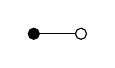
\begin{tikzpicture}[scale=1]
	\draw[line width=0.5](0,0)--(0.6,0);
	\filldraw[fill=black](0,0)circle(2pt);
	\filldraw[fill=white](0.6,0)circle(2pt);
\end{tikzpicture}
}

\unitlength1cm
\newcommand{\FTV}
{
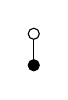
\begin{tikzpicture}[>=latex', scale=1]
	\draw[line width=0.5](0,0.2)--(0,-0.2);
	\filldraw[fill=white] (0,0.2)circle (2pt);
	\filldraw[fill=black](0,-0.2)circle (2pt);
\end{tikzpicture}
}

